% si-appendix.tex -- PNAS SI Appendix (standalone document)
% Training-Free Generation of Protein Sequences via Stochastic Attention
\documentclass[9pt]{article}

\usepackage[utf8]{inputenc}
\usepackage[T1]{fontenc}
\usepackage[scaled]{helvet}
\renewcommand{\familydefault}{\sfdefault}
\usepackage{amsmath,amssymb,amsfonts}
\usepackage{graphicx}
\usepackage{booktabs}
\usepackage{multirow}
\usepackage[colorlinks=true,allcolors=blue]{hyperref}
\usepackage[numbers,sort&compress]{natbib}
\usepackage{algorithm}
\usepackage[noend]{algpseudocode}
\usepackage[margin=1in]{geometry}
\usepackage{caption}

% SI numbering: S-prefixed figures, tables, sections
\renewcommand{\thefigure}{S\arabic{figure}}
\renewcommand{\thetable}{S\arabic{table}}
\renewcommand{\thesection}{S\arabic{section}}
\renewcommand{\theequation}{S\arabic{equation}}

\title{SI Appendix:\\Training-Free Generation of Protein Sequences from Small Family Alignments via Stochastic Attention}
\author{Jeffrey D. Varner\\
R.F. Smith School of Chemical and Biomolecular Engineering, Cornell University}
\date{}

\begin{document}
\maketitle

%% ═══════════════════════════════════════════════════════════════════════
%% S1. Amino Acid Composition Profiles
%% ═══════════════════════════════════════════════════════════════════════
\section{Amino Acid Composition Profiles}\label{si:aa-freq}

We compared the per-position amino acid frequency profiles of the stored seed sequences and SA-generated sequences for the RRM family (PF00076, Fig.~\ref{fig:aa-freq}). The generated ensemble faithfully reproduces the conservation pattern of the family: strongly conserved positions retain high frequency in the generated output, while variable positions display a similar breadth of amino acid usage.

\begin{figure}[ht]
\centering
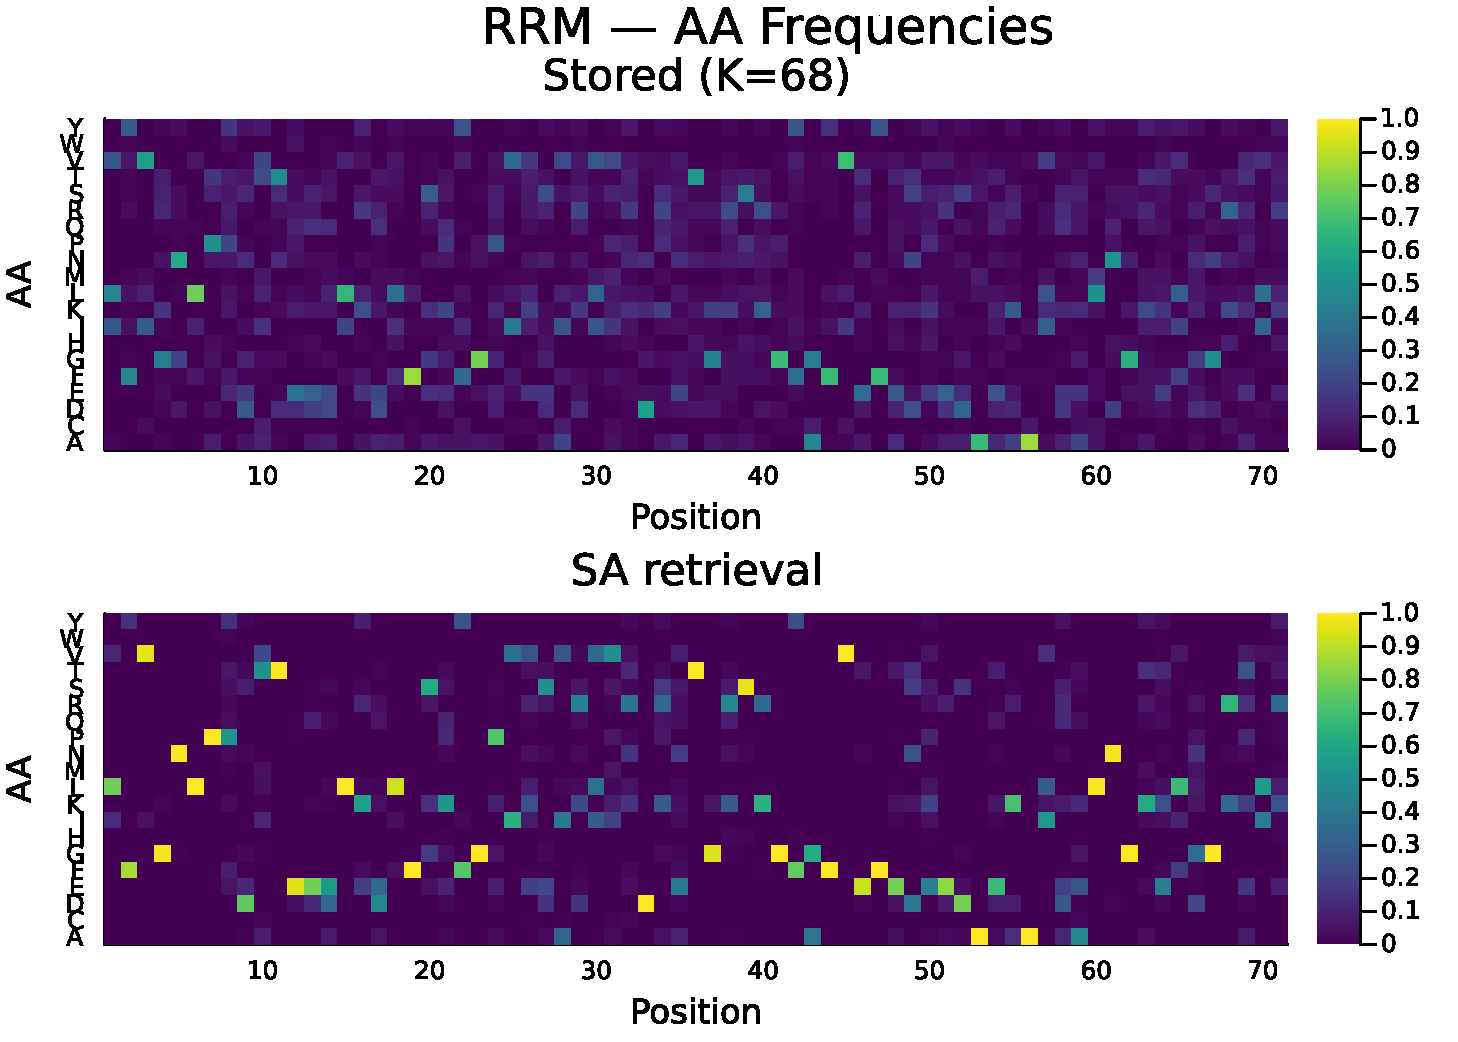
\includegraphics[width=0.9\textwidth]{figs/aa_freq_example.pdf}
\caption{Per-position amino acid frequency profiles for the RRM family (PF00076). \textbf{Top:} stored seed sequences ($K{=}68$). \textbf{Bottom:} SA-generated sequences ($S{=}150$, retrieval regime).}
\label{fig:aa-freq}
\end{figure}

%% ═══════════════════════════════════════════════════════════════════════
%% S2. Generation Metrics (Full Table)
%% ═══════════════════════════════════════════════════════════════════════
\section{Generation Metrics}\label{si:generation-metrics}

Table~\ref{tab:results} reports the full generation metrics for all eight Pfam families across five sampling conditions: SA generation ($\beta \approx 2\beta^*$), SA retrieval ($\beta \approx 20\beta^*$), bootstrap resampling, Gaussian perturbation, and convex combination.

\begin{table}[ht]
\centering
\caption{Generation metrics across eight Pfam families (mean $\pm$ SE). SA gen: generation regime ($\beta \approx 2\beta^*$). SA ret: retrieval regime ($\beta \approx 20\beta^*$). BS: bootstrap. GP: Gaussian perturbation. CC: convex combination.}
\label{tab:results}
\small
\begin{tabular}{@{}llccc@{}}
\toprule
Family & Method & KL$_{\mathrm{AA}}$ $(\downarrow)$ & Novelty $(\uparrow)$ & SeqID $(\downarrow)$ \\
\midrule
\multirow{5}{*}{RRM}
 & SA gen  & $\mathbf{0.060 \pm 0.005}$ & $\mathbf{0.513 \pm 0.011}$ & $\mathbf{0.538 \pm 0.006}$ \\
 & SA ret  & $0.107 \pm 0.010$ & $0.334 \pm 0.020$ & $0.616 \pm 0.012$ \\
 & BS      & $0.133 \pm 0.006$ & $0.000 \pm 0.000$ & $0.645 \pm 0.004$ \\
 & GP      & $0.132 \pm 0.005$ & $0.008 \pm 0.000$ & $0.633 \pm 0.006$ \\
 & CC      & $2.091 \pm 0.000$ & $0.510 \pm 0.009$ & $0.562 \pm 0.000$ \\
\midrule
\multirow{5}{*}{SH3}
 & SA gen  & $0.036 \pm 0.004$ & $\mathbf{0.471 \pm 0.012}$ & $\mathbf{0.593 \pm 0.006}$ \\
 & SA ret  & $0.035 \pm 0.004$ & $0.213 \pm 0.012$ & $0.722 \pm 0.011$ \\
 & BS      & $\mathbf{0.030 \pm 0.003}$ & $0.000 \pm 0.000$ & $0.772 \pm 0.006$ \\
 & GP      & $\mathbf{0.030 \pm 0.003}$ & $0.006 \pm 0.000$ & $0.752 \pm 0.006$ \\
 & CC      & $0.798 \pm 0.012$ & $0.474 \pm 0.008$ & $0.601 \pm 0.002$ \\
\midrule
\multirow{5}{*}{WW}
 & SA gen  & $\mathbf{0.008 \pm 0.002}$ & $\mathbf{0.653 \pm 0.006}$ & $\mathbf{0.562 \pm 0.005}$ \\
 & SA ret  & $0.046 \pm 0.013$ & $0.354 \pm 0.016$ & $0.763 \pm 0.011$ \\
 & BS      & $0.024 \pm 0.003$ & $0.000 \pm 0.000$ & $0.823 \pm 0.005$ \\
 & GP      & $0.029 \pm 0.004$ & $0.017 \pm 0.000$ & $0.809 \pm 0.006$ \\
 & CC      & $1.375 \pm 0.092$ & $0.637 \pm 0.004$ & $0.766 \pm 0.001$ \\
\midrule
\multirow{5}{*}{Kunitz}
 & SA gen  & $\mathbf{0.013 \pm 0.002}$ & $\mathbf{0.557 \pm 0.009}$ & $\mathbf{0.607 \pm 0.004}$ \\
 & SA ret  & $0.037 \pm 0.003$ & $0.257 \pm 0.016$ & $0.760 \pm 0.012$ \\
 & BS      & $0.023 \pm 0.002$ & $0.000 \pm 0.000$ & $0.834 \pm 0.004$ \\
 & GP      & $0.024 \pm 0.002$ & $0.010 \pm 0.000$ & $0.844 \pm 0.004$ \\
 & CC      & $0.721 \pm 0.013$ & $0.546 \pm 0.007$ & $0.590 \pm 0.001$ \\
\midrule
\multirow{5}{*}{zf-C2H2}
 & SA gen  & $0.013 \pm 0.028$ & $\mathbf{0.596 \pm 0.010}$ & $\mathbf{0.557 \pm 0.007}$ \\
 & SA ret  & $0.021 \pm 0.010$ & $0.167 \pm 0.014$ & $0.848 \pm 0.013$ \\
 & BS      & $\mathbf{0.007 \pm 0.002}$ & $0.000 \pm 0.000$ & $0.938 \pm 0.004$ \\
 & GP      & $\mathbf{0.007 \pm 0.002}$ & $0.011 \pm 0.000$ & $0.940 \pm 0.004$ \\
 & CC      & $2.346 \pm 0.060$ & $0.580 \pm 0.006$ & $0.600 \pm 0.001$ \\
\midrule
\multirow{5}{*}{PDZ}
 & SA gen  & $\mathbf{0.038 \pm 0.010}$ & $\mathbf{0.418 \pm 0.009}$ & $\mathbf{0.543 \pm 0.005}$ \\
 & SA ret  & $0.059 \pm 0.016$ & $0.236 \pm 0.017$ & $0.626 \pm 0.014$ \\
 & BS      & $0.041 \pm 0.002$ & $0.000 \pm 0.000$ & $0.642 \pm 0.009$ \\
 & GP      & $0.045 \pm 0.003$ & $0.006 \pm 0.000$ & $0.648 \pm 0.007$ \\
 & CC      & $0.760 \pm 0.030$ & $0.443 \pm 0.010$ & $0.523 \pm 0.003$ \\
\midrule
\multirow{5}{*}{Pkinase}
 & SA gen  & $\mathbf{0.044 \pm 0.003}$ & $\mathbf{0.397 \pm 0.010}$ & $\mathbf{0.514 \pm 0.003}$ \\
 & SA ret  & $0.067 \pm 0.010$ & $0.173 \pm 0.017$ & $0.535 \pm 0.012$ \\
 & BS      & $0.078 \pm 0.005$ & $0.000 \pm 0.000$ & $0.547 \pm 0.007$ \\
 & GP      & $0.069 \pm 0.005$ & $0.006 \pm 0.001$ & $0.540 \pm 0.007$ \\
 & CC      & $1.640 \pm 0.030$ & $0.364 \pm 0.008$ & $0.531 \pm 0.001$ \\
\midrule
\multirow{5}{*}{Def.\_beta}
 & SA gen  & $\mathbf{0.024 \pm 0.005}$ & $\mathbf{0.400 \pm 0.012}$ & $\mathbf{0.656 \pm 0.007}$ \\
 & SA ret  & $0.030 \pm 0.007$ & $0.190 \pm 0.016$ & $0.788 \pm 0.013$ \\
 & BS      & $0.038 \pm 0.003$ & $0.000 \pm 0.000$ & $0.780 \pm 0.007$ \\
 & GP      & $0.035 \pm 0.003$ & $0.009 \pm 0.001$ & $0.768 \pm 0.006$ \\
 & CC      & $0.590 \pm 0.020$ & $0.390 \pm 0.010$ & $0.638 \pm 0.002$ \\
\bottomrule
\end{tabular}
\end{table}

%% ═══════════════════════════════════════════════════════════════════════
%% S3. Scaling Study
%% ═══════════════════════════════════════════════════════════════════════
\section{Scaling Study}\label{si:scaling}

To characterize how generation quality degrades with decreasing family size, we subsampled the WW domain ($K{=}420$) at $K \in \{20, 50, 100, 200, 400\}$ with five independent replicates per condition (Fig.~\ref{fig:scaling}). Stochastic attention maintained low KL divergence across the entire range ($0.019 \pm 0.008$ at $K{=}20$), while novelty increased with $K$ (from $0.47$ to $0.74$).

\begin{figure}[ht]
\centering
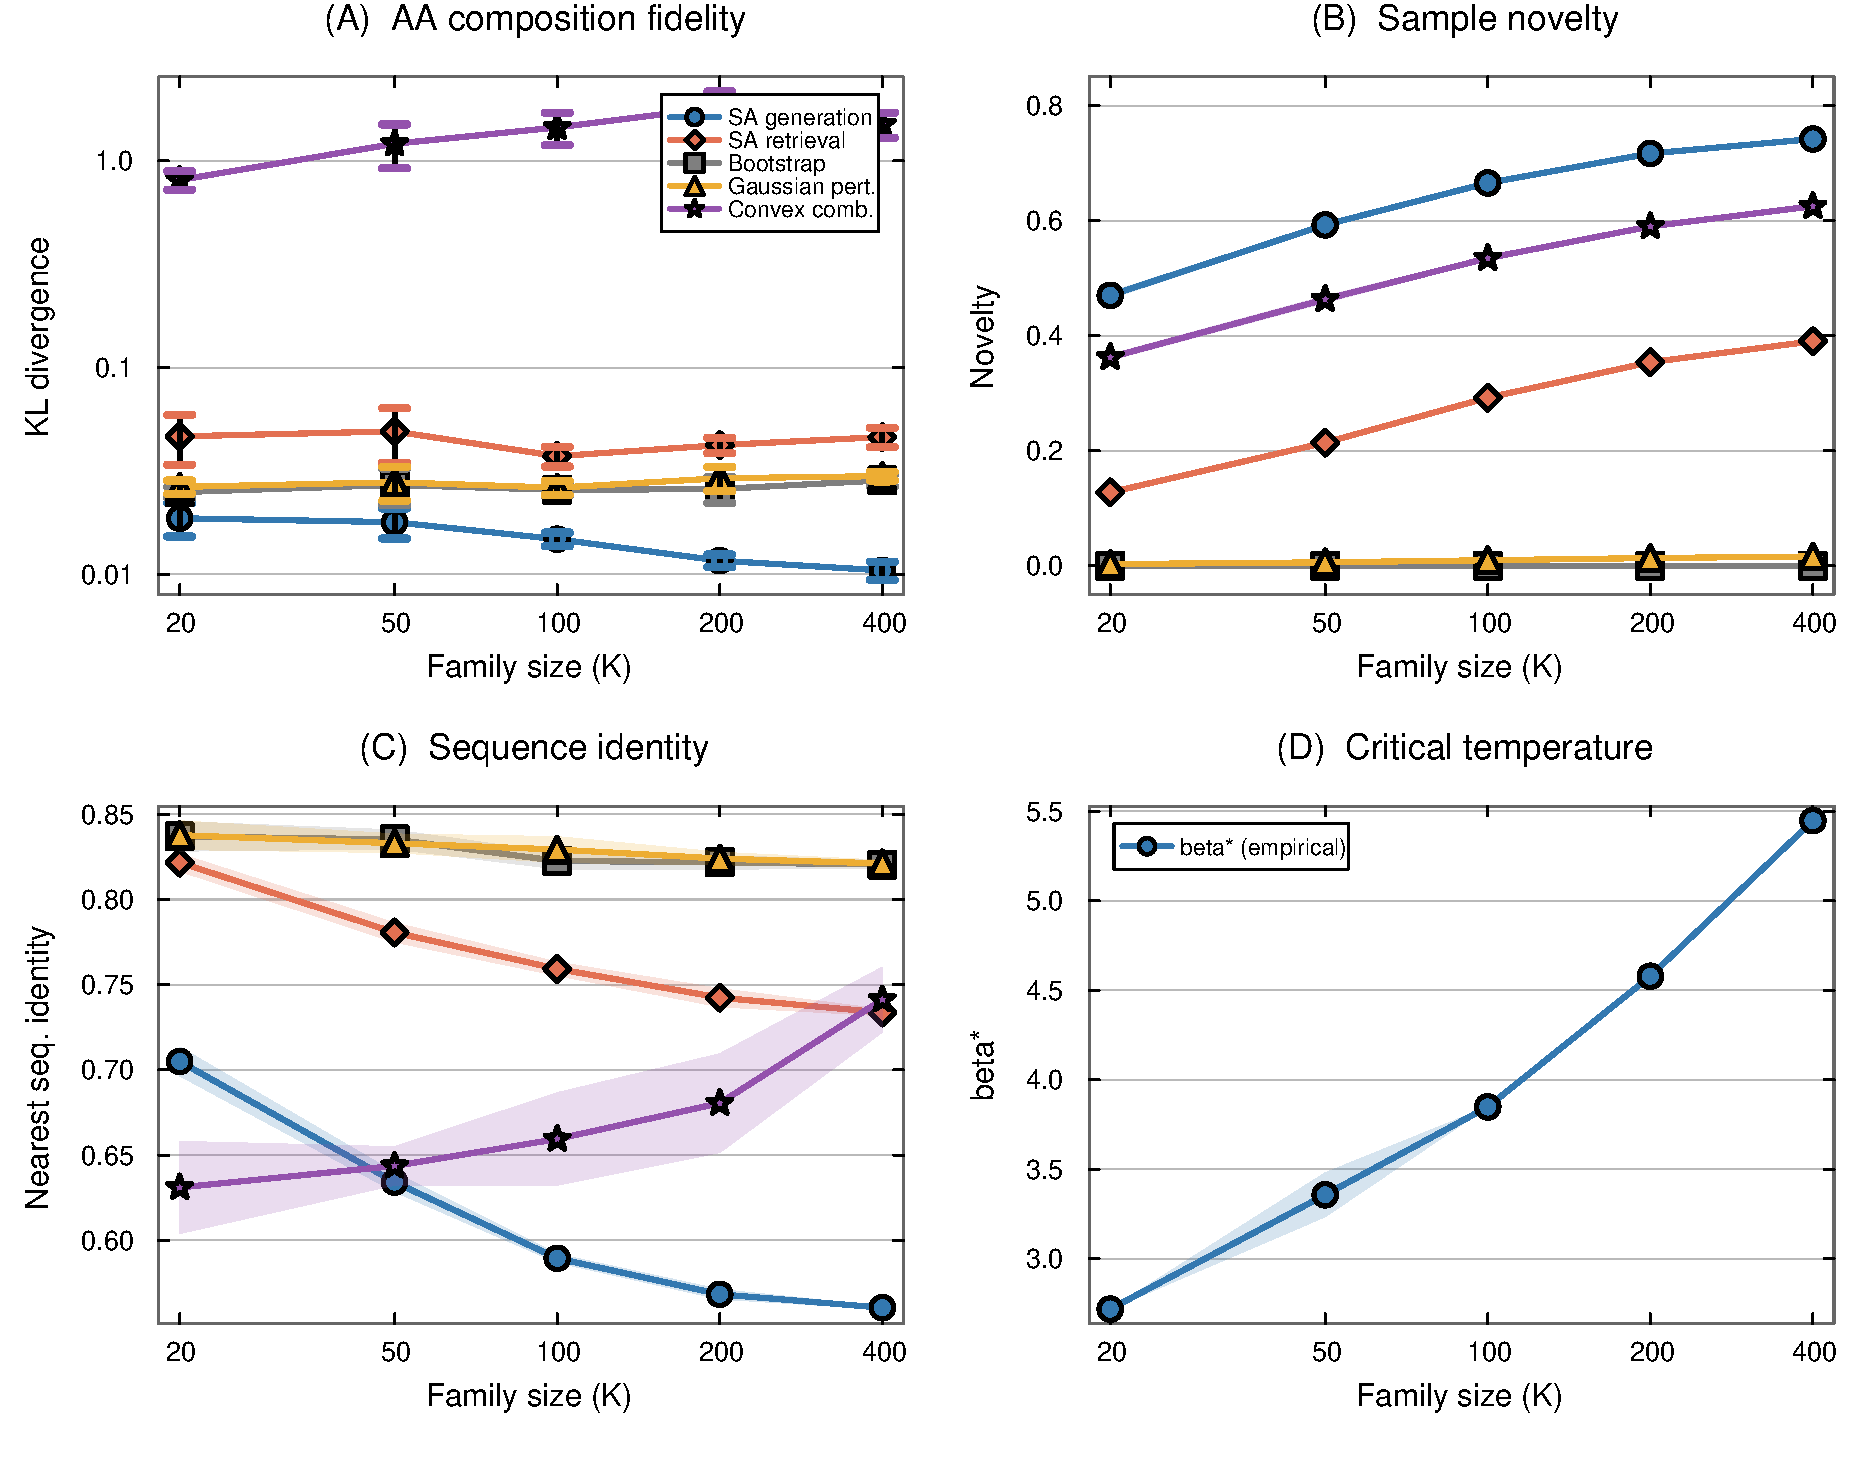
\includegraphics[width=\textwidth]{figs/scaling_composite.pdf}
\caption{Scaling study: WW domain subsampled at $K \in \{20, 50, 100, 200, 400\}$ with five independent replicates. \textbf{(A)}~KL divergence. \textbf{(B)}~Novelty. \textbf{(C)}~Nearest sequence identity. \textbf{(D)}~Critical temperature $\beta^*$. Shaded regions: $\pm 1$ SE.}
\label{fig:scaling}
\end{figure}

%% ═══════════════════════════════════════════════════════════════════════
%% S4. Multi-Family Scaling at K=20
%% ═══════════════════════════════════════════════════════════════════════
\section{Multi-Family Scaling at \texorpdfstring{$K{=}20$}{K=20}}\label{si:multifamily-scaling}

To test generality, we subsampled three additional families to $K{=}20$ with five replicates each (Table~\ref{tab:multifamily-k20}).

\begin{table}[ht]
\centering
\small
\caption{SA generation quality at $K{=}20$ across four Pfam families (five independent subsamples each). Values: mean $\pm$ SD.}
\label{tab:multifamily-k20}
\begin{tabular}{lcccccc}
\toprule
Family & $K_{\mathrm{full}}$ & $L$ & $d_{\mathrm{PCA}}$ & KL & Novelty & Seq.\ ID \\
\midrule
SH3     & 55  & 48 & 17--18 & $0.026 \pm 0.003$ & $0.46 \pm 0.01$ & $0.67 \pm 0.01$ \\
Kunitz  & 99  & 53 & 17--18 & $0.020 \pm 0.004$ & $0.47 \pm 0.01$ & $0.72 \pm 0.01$ \\
zf-C2H2 & 151 & 23 & 18     & $0.013 \pm 0.004$ & $0.47 \pm 0.01$ & $0.73 \pm 0.00$ \\
WW      & 420 & 31 & 17--18 & $0.019 \pm 0.008$ & $0.47 \pm 0.01$ & $0.71 \pm 0.02$ \\
\bottomrule
\end{tabular}
\end{table}

%% ═══════════════════════════════════════════════════════════════════════
%% S5. AlphaFold2 Cross-Validation
%% ═══════════════════════════════════════════════════════════════════════
\section{AlphaFold2 Cross-Validation}\label{si:af2}

AlphaFold2 cross-validation corroborated the ESMFold findings across all eight families (Fig.~\ref{fig:structure-esmfold-af2}). TM-scores were significantly higher for SA generation in all eight families ($p < 0.05$; Cohen's $d{=}0.47$--$1.73$). The concordance between two independent structure predictors (TM-score $r{=}0.999$) strengthens the computational evidence that SA-generated sequences are predicted to adopt the correct fold (Fig.~\ref{fig:esmfold-af2-concordance}).

\begin{figure}[ht]
\centering
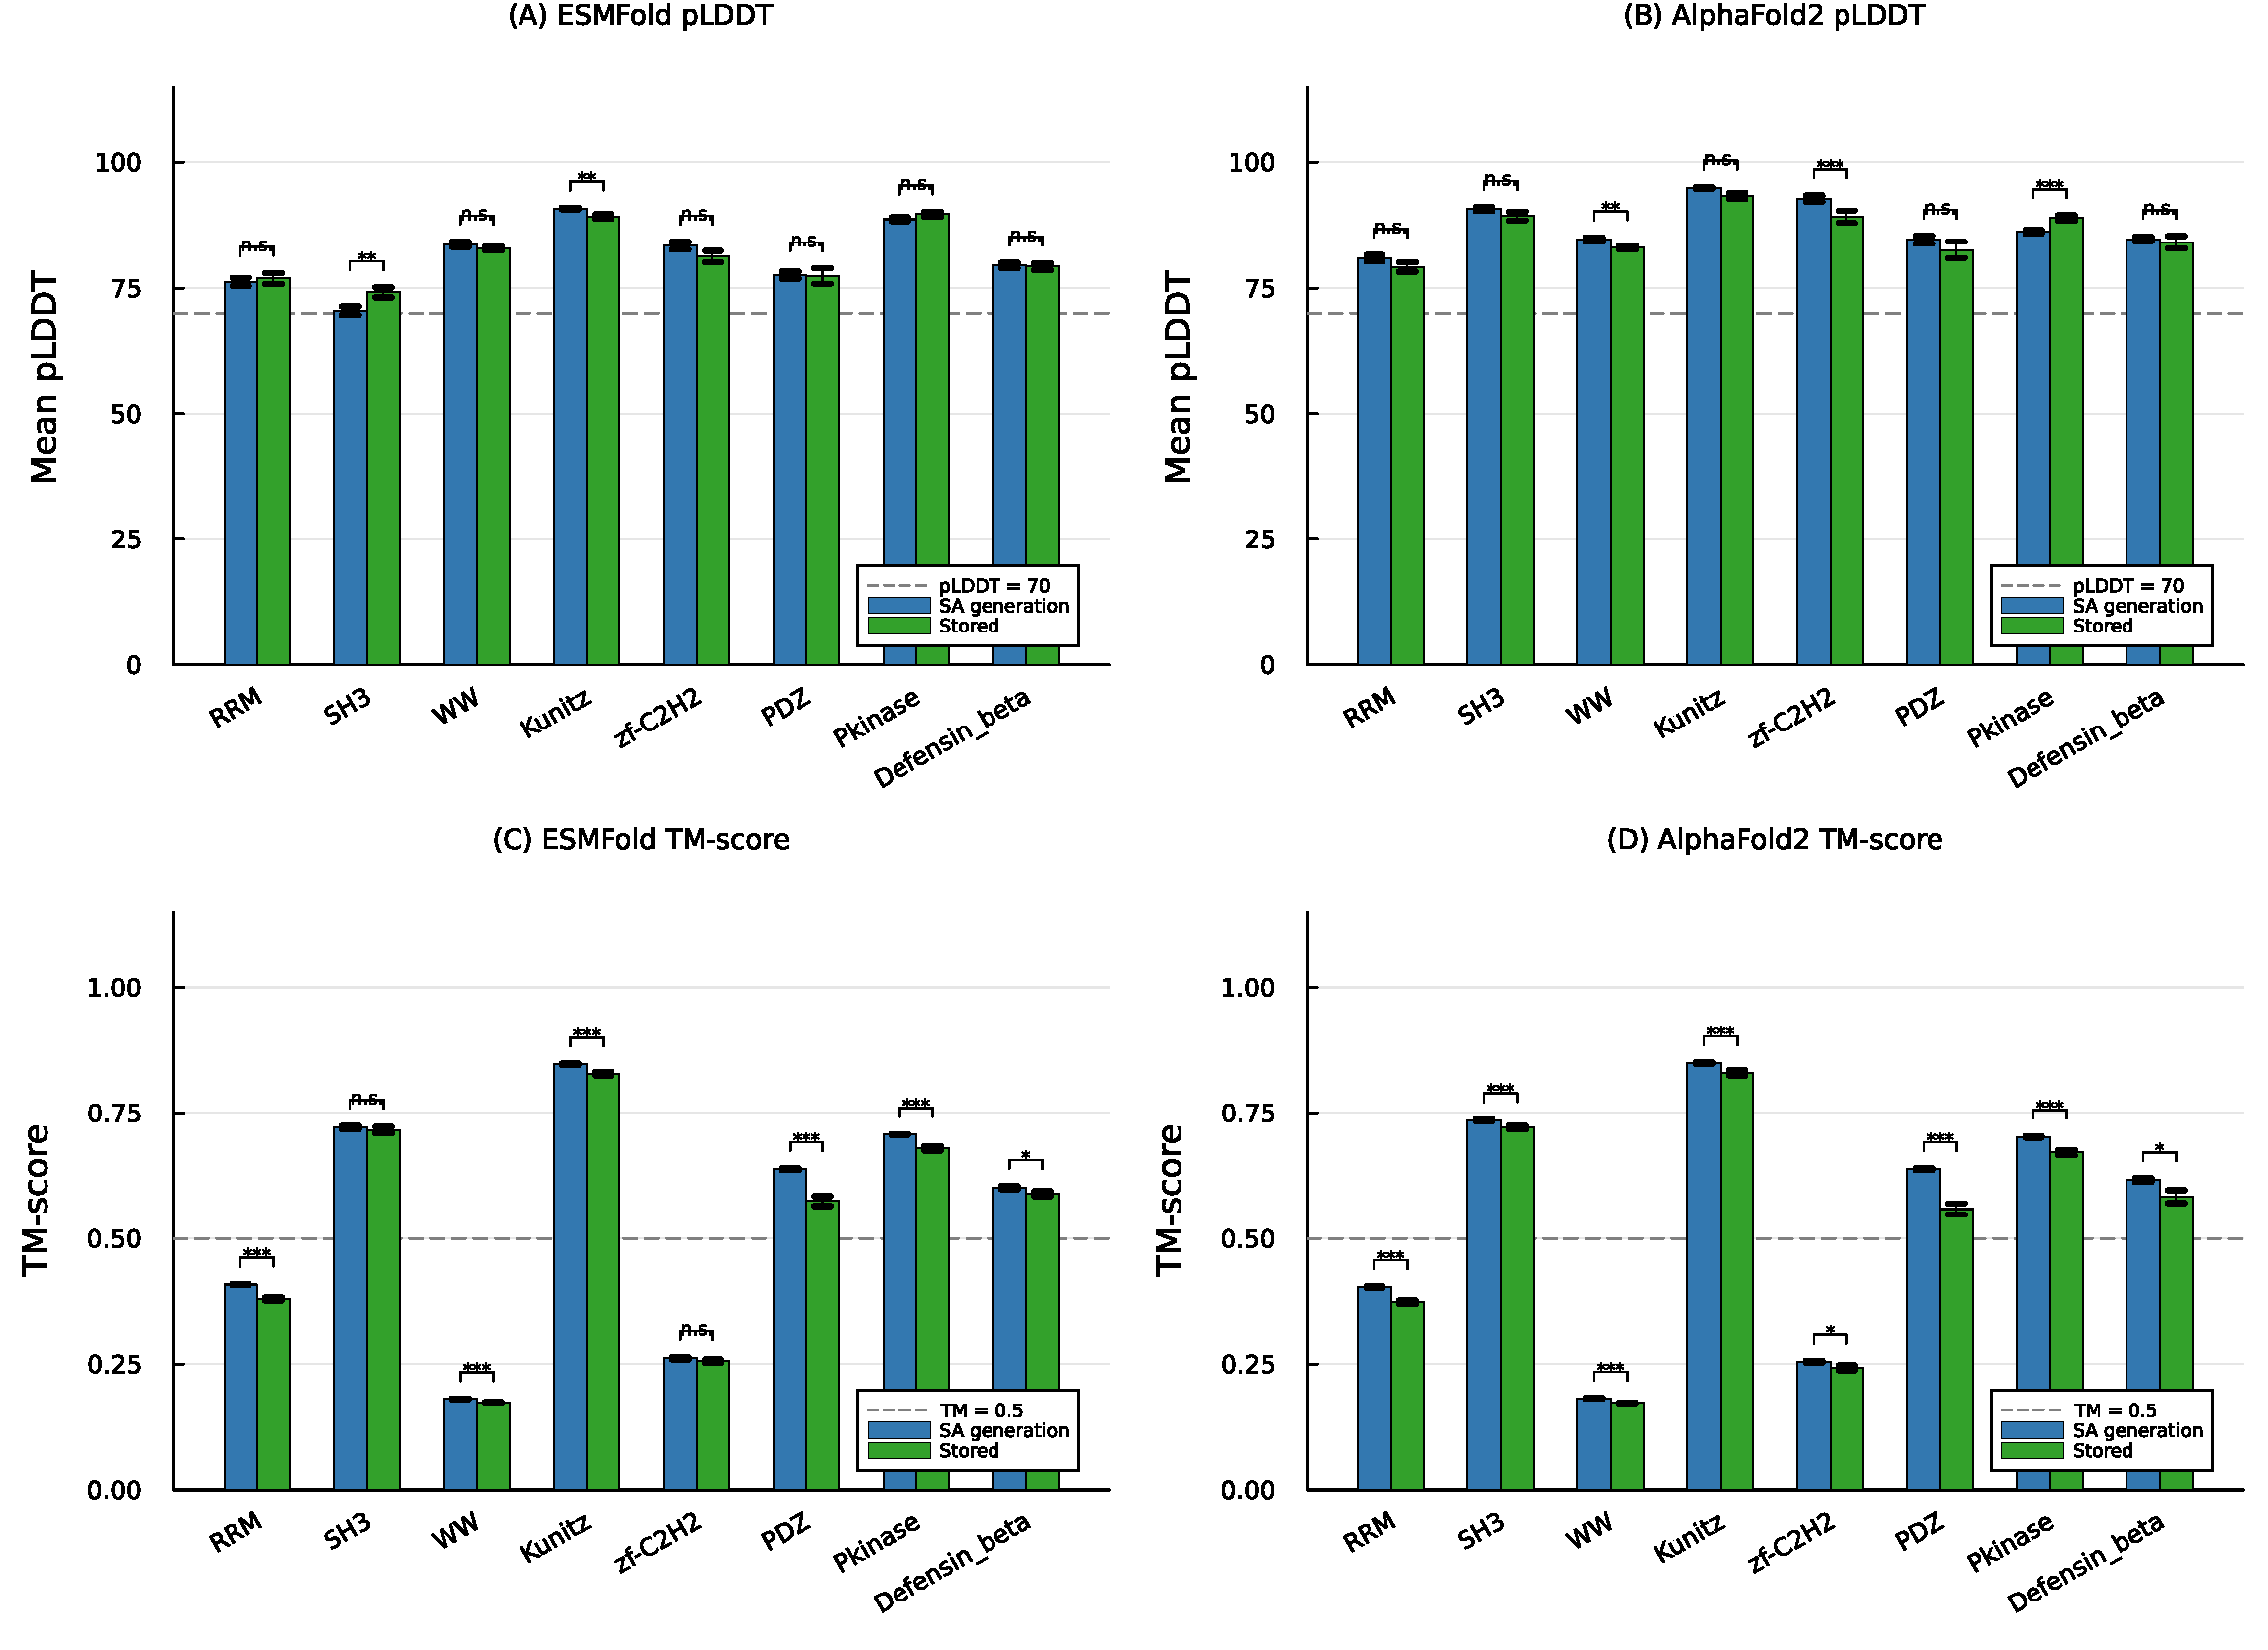
\includegraphics[width=\textwidth]{figs/structure_validation_esmfold_af2.pdf}
\caption{AlphaFold2 cross-validation of structure predictions across all eight families. pLDDT and TM-score comparisons between SA-generated and stored sequences.}
\label{fig:structure-esmfold-af2}
\end{figure}

\begin{figure}[ht]
\centering
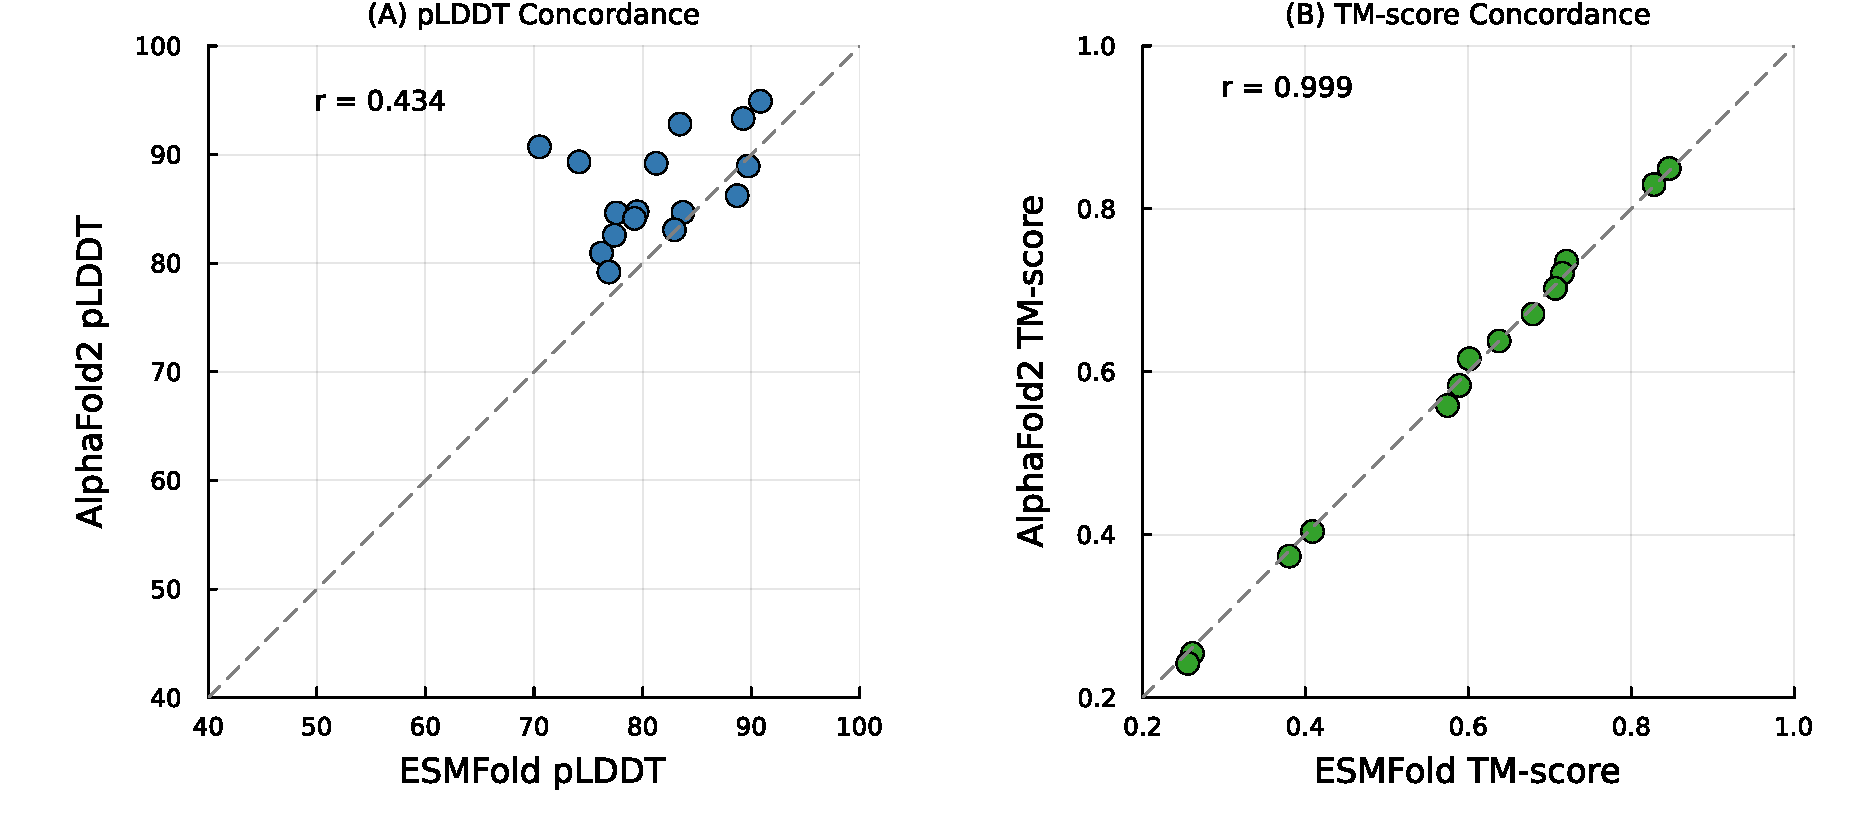
\includegraphics[width=0.7\textwidth]{figs/esmfold_af2_concordance.pdf}
\caption{Concordance between ESMFold and AlphaFold2 TM-scores across all eight families.}
\label{fig:esmfold-af2-concordance}
\end{figure}

%% ═══════════════════════════════════════════════════════════════════════
%% S6. Sequence Analysis (Kunitz)
%% ═══════════════════════════════════════════════════════════════════════
\section{Sequence-Level Analysis}\label{si:sequence-analysis}

We aligned the five highest-confidence SA-generated Kunitz domain sequences against the family consensus (Fig.~\ref{fig:sequence-analysis}). All five sequences preserved every highly conserved position (11 of 11 positions with $>90\%$ conservation) and all six cysteines, while introducing 17--25 substitutions concentrated at variable positions. Per-position Shannon entropy correlated strongly with the stored MSA ($r{=}0.968$).

\begin{figure}[ht]
\centering
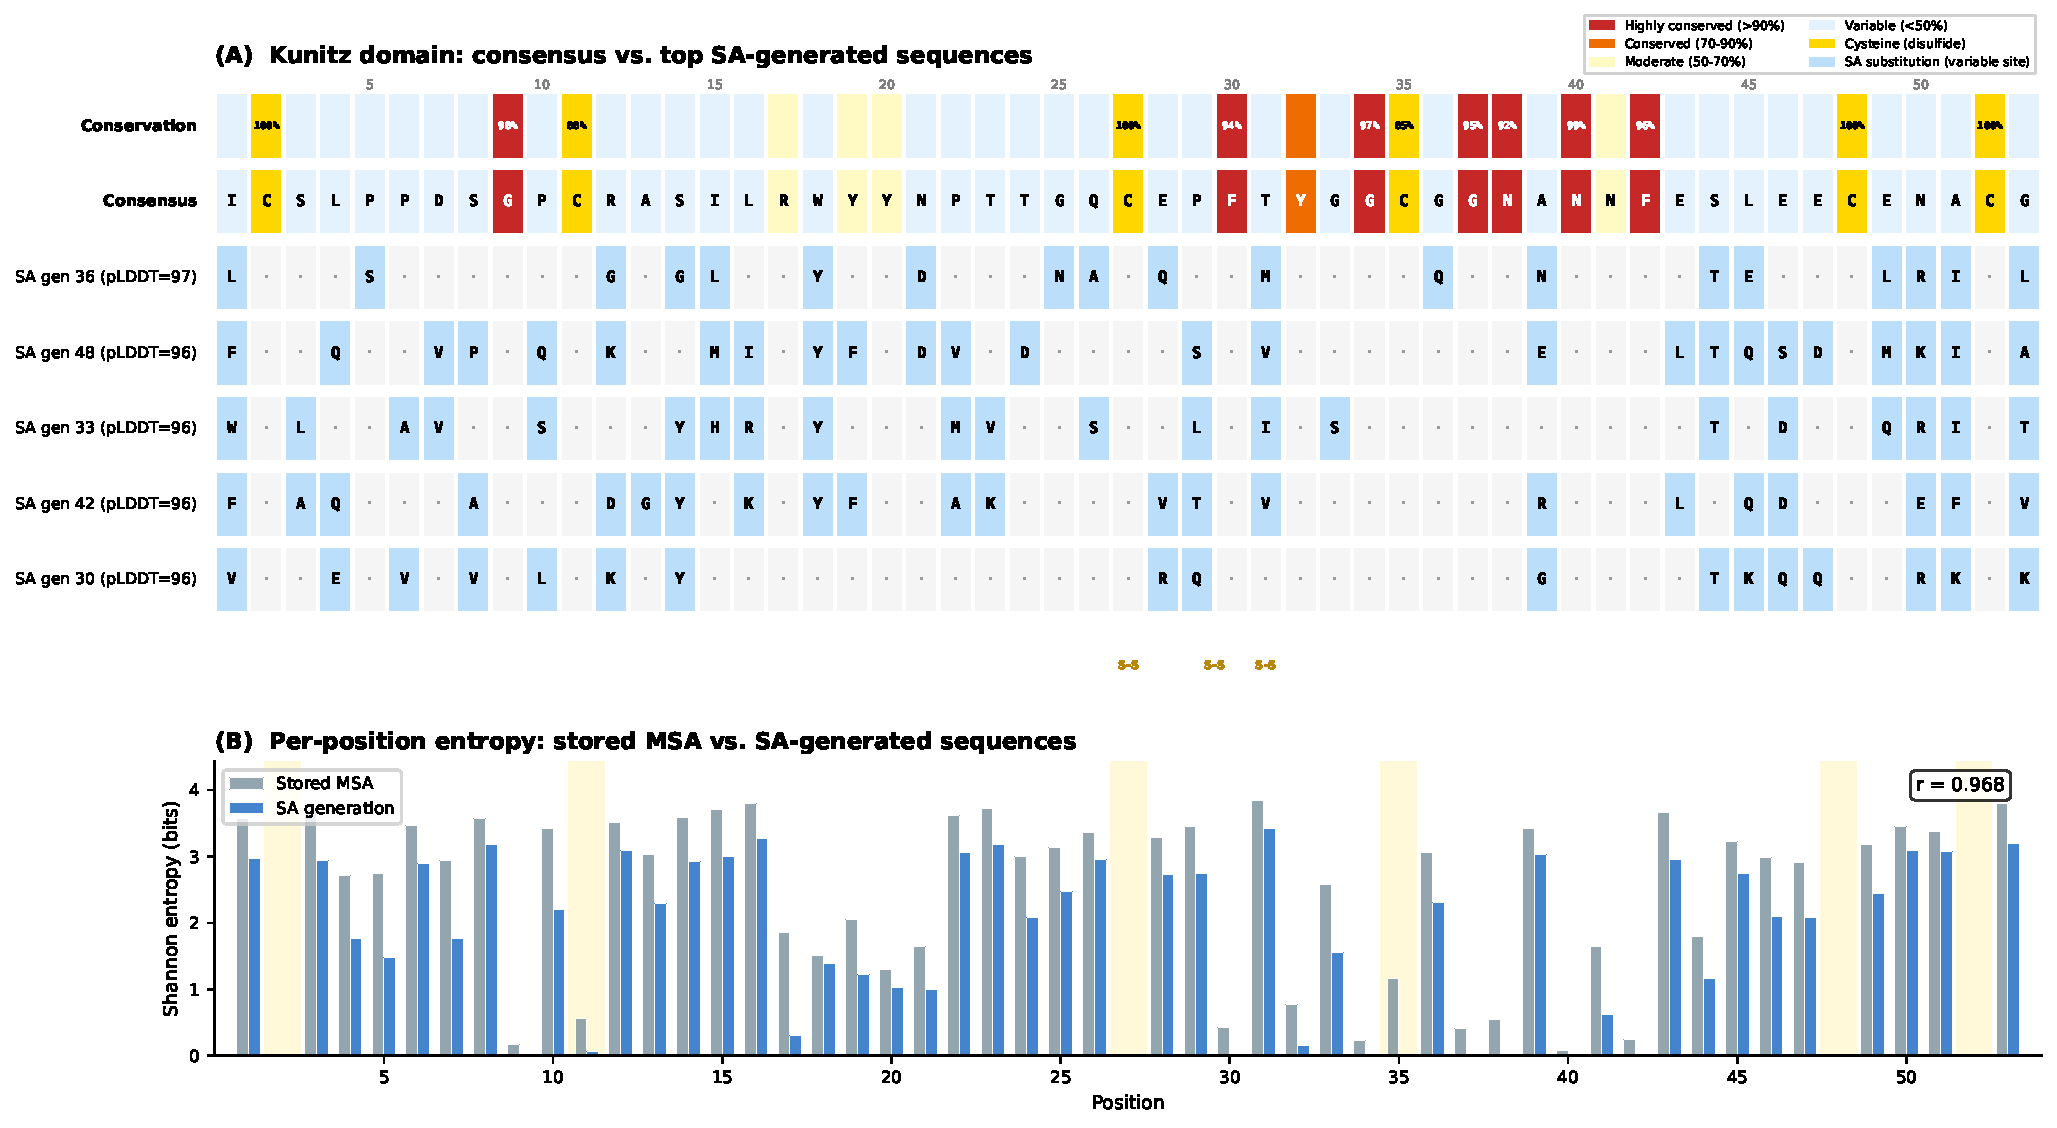
\includegraphics[width=\textwidth]{figs/sequence_analysis_kunitz.pdf}
\caption{Sequence-level analysis of SA-generated Kunitz domain sequences. \textbf{(A)}~Alignment colored by conservation level. \textbf{(B)}~Per-position Shannon entropy correlation ($r{=}0.968$).}
\label{fig:sequence-analysis}
\end{figure}

%% ═══════════════════════════════════════════════════════════════════════
%% S7. Pairwise Mutual Information
%% ═══════════════════════════════════════════════════════════════════════
\section{Pairwise Mutual Information Analysis}\label{si:mi}

SA-generated sequences preserved the pairwise MI landscape of the stored alignment (Pearson $r{=}0.53$--$0.92$ across seven families), consistently exceeding profile HMMs ($r{=}0.07$--$0.83$).

\begin{figure}[ht]
\centering
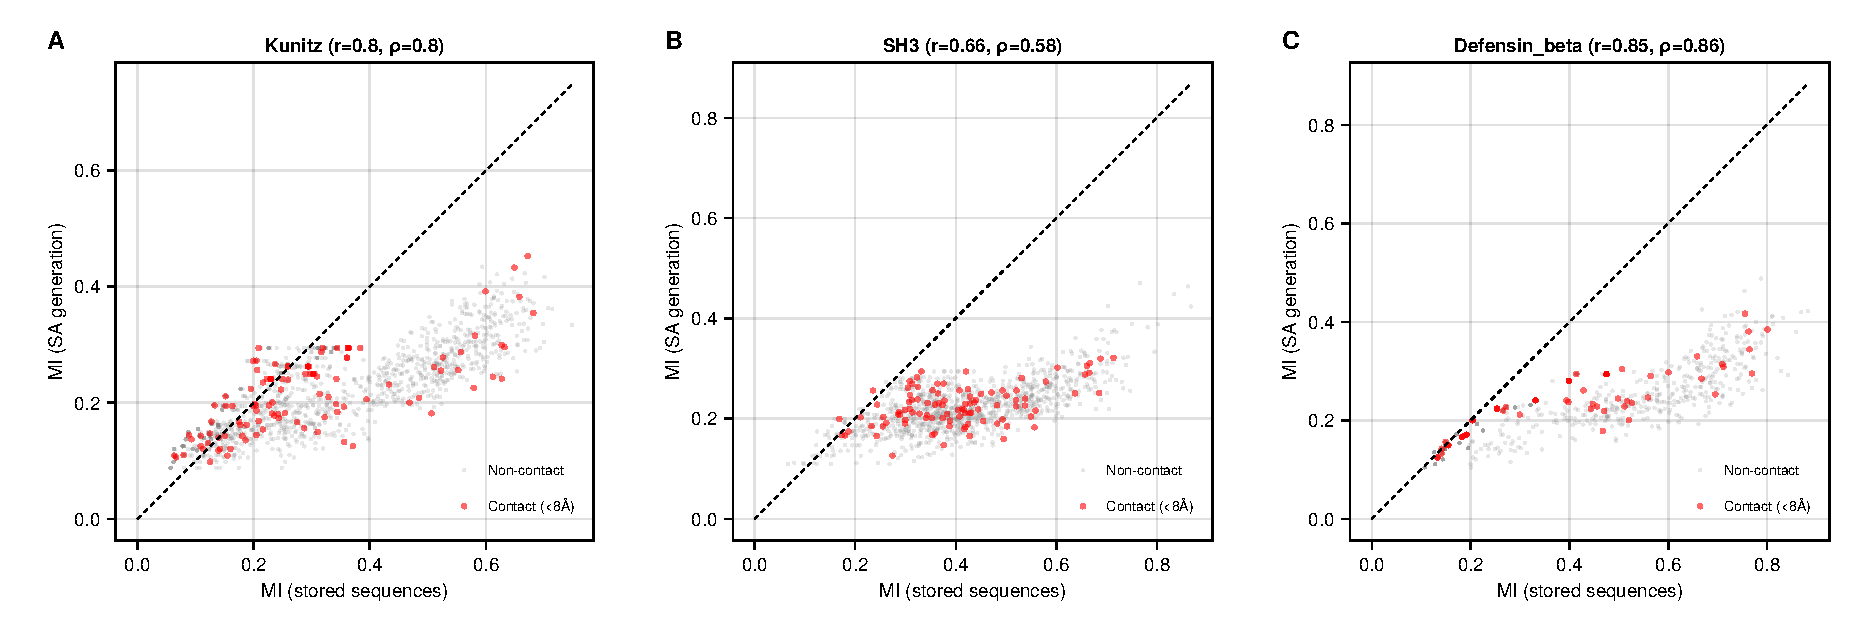
\includegraphics[width=\textwidth]{figs/mi_covariation_scatter.pdf}
\caption{Pairwise mutual information: stored vs.\ SA-generated for each family.}
\label{fig:mi-scatter}
\end{figure}

\begin{figure}[ht]
\centering
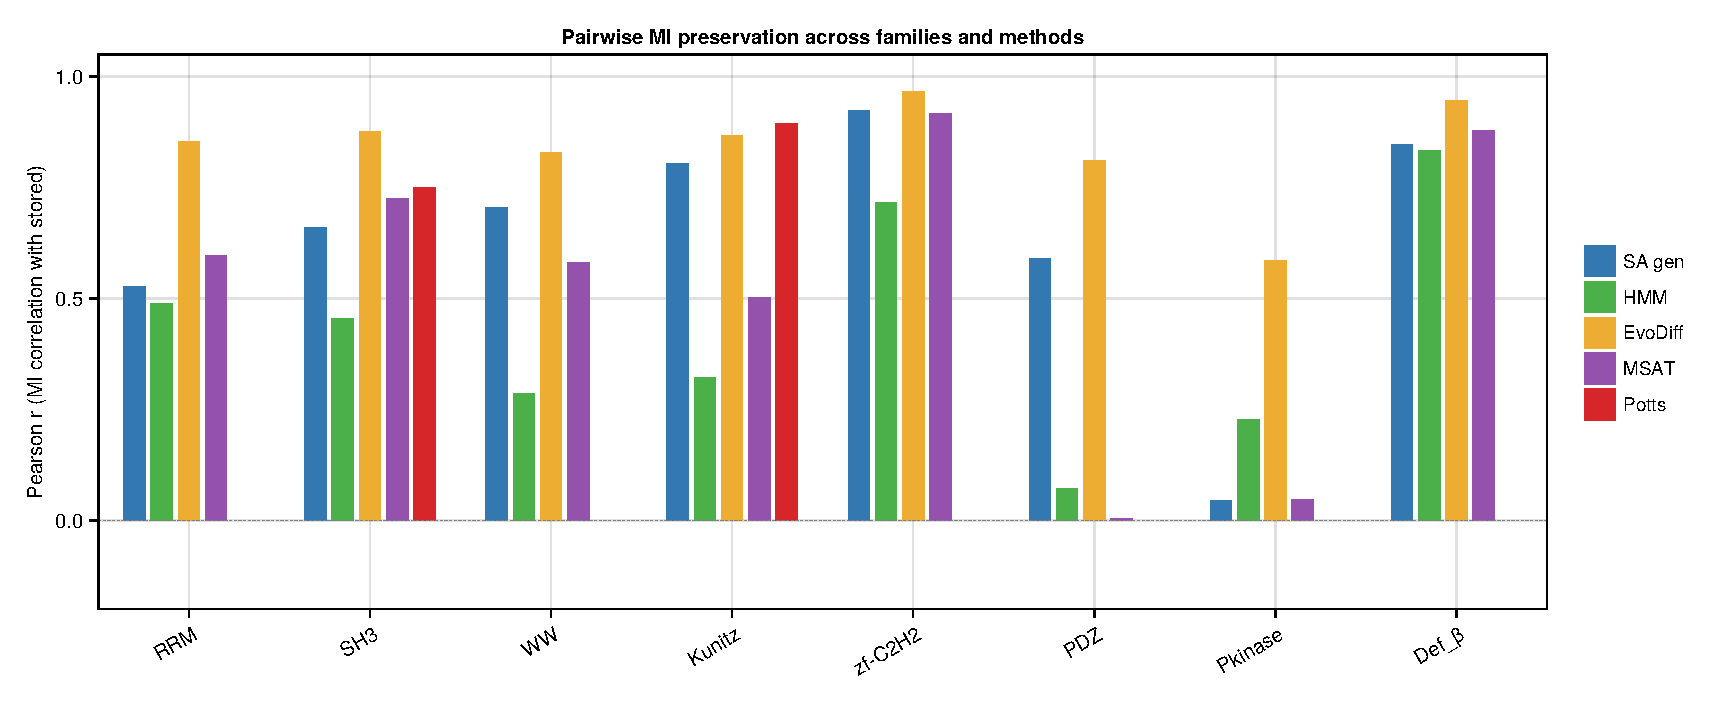
\includegraphics[width=\textwidth]{figs/mi_covariation_barplot.pdf}
\caption{MI Pearson correlation by method across families.}
\label{fig:mi-barplot}
\end{figure}

%% ═══════════════════════════════════════════════════════════════════════
%% S8. Beta-Star Analysis
%% ═══════════════════════════════════════════════════════════════════════
\section{Critical Temperature Analysis}\label{si:beta-star-analysis}

\begin{figure}[ht]
\centering
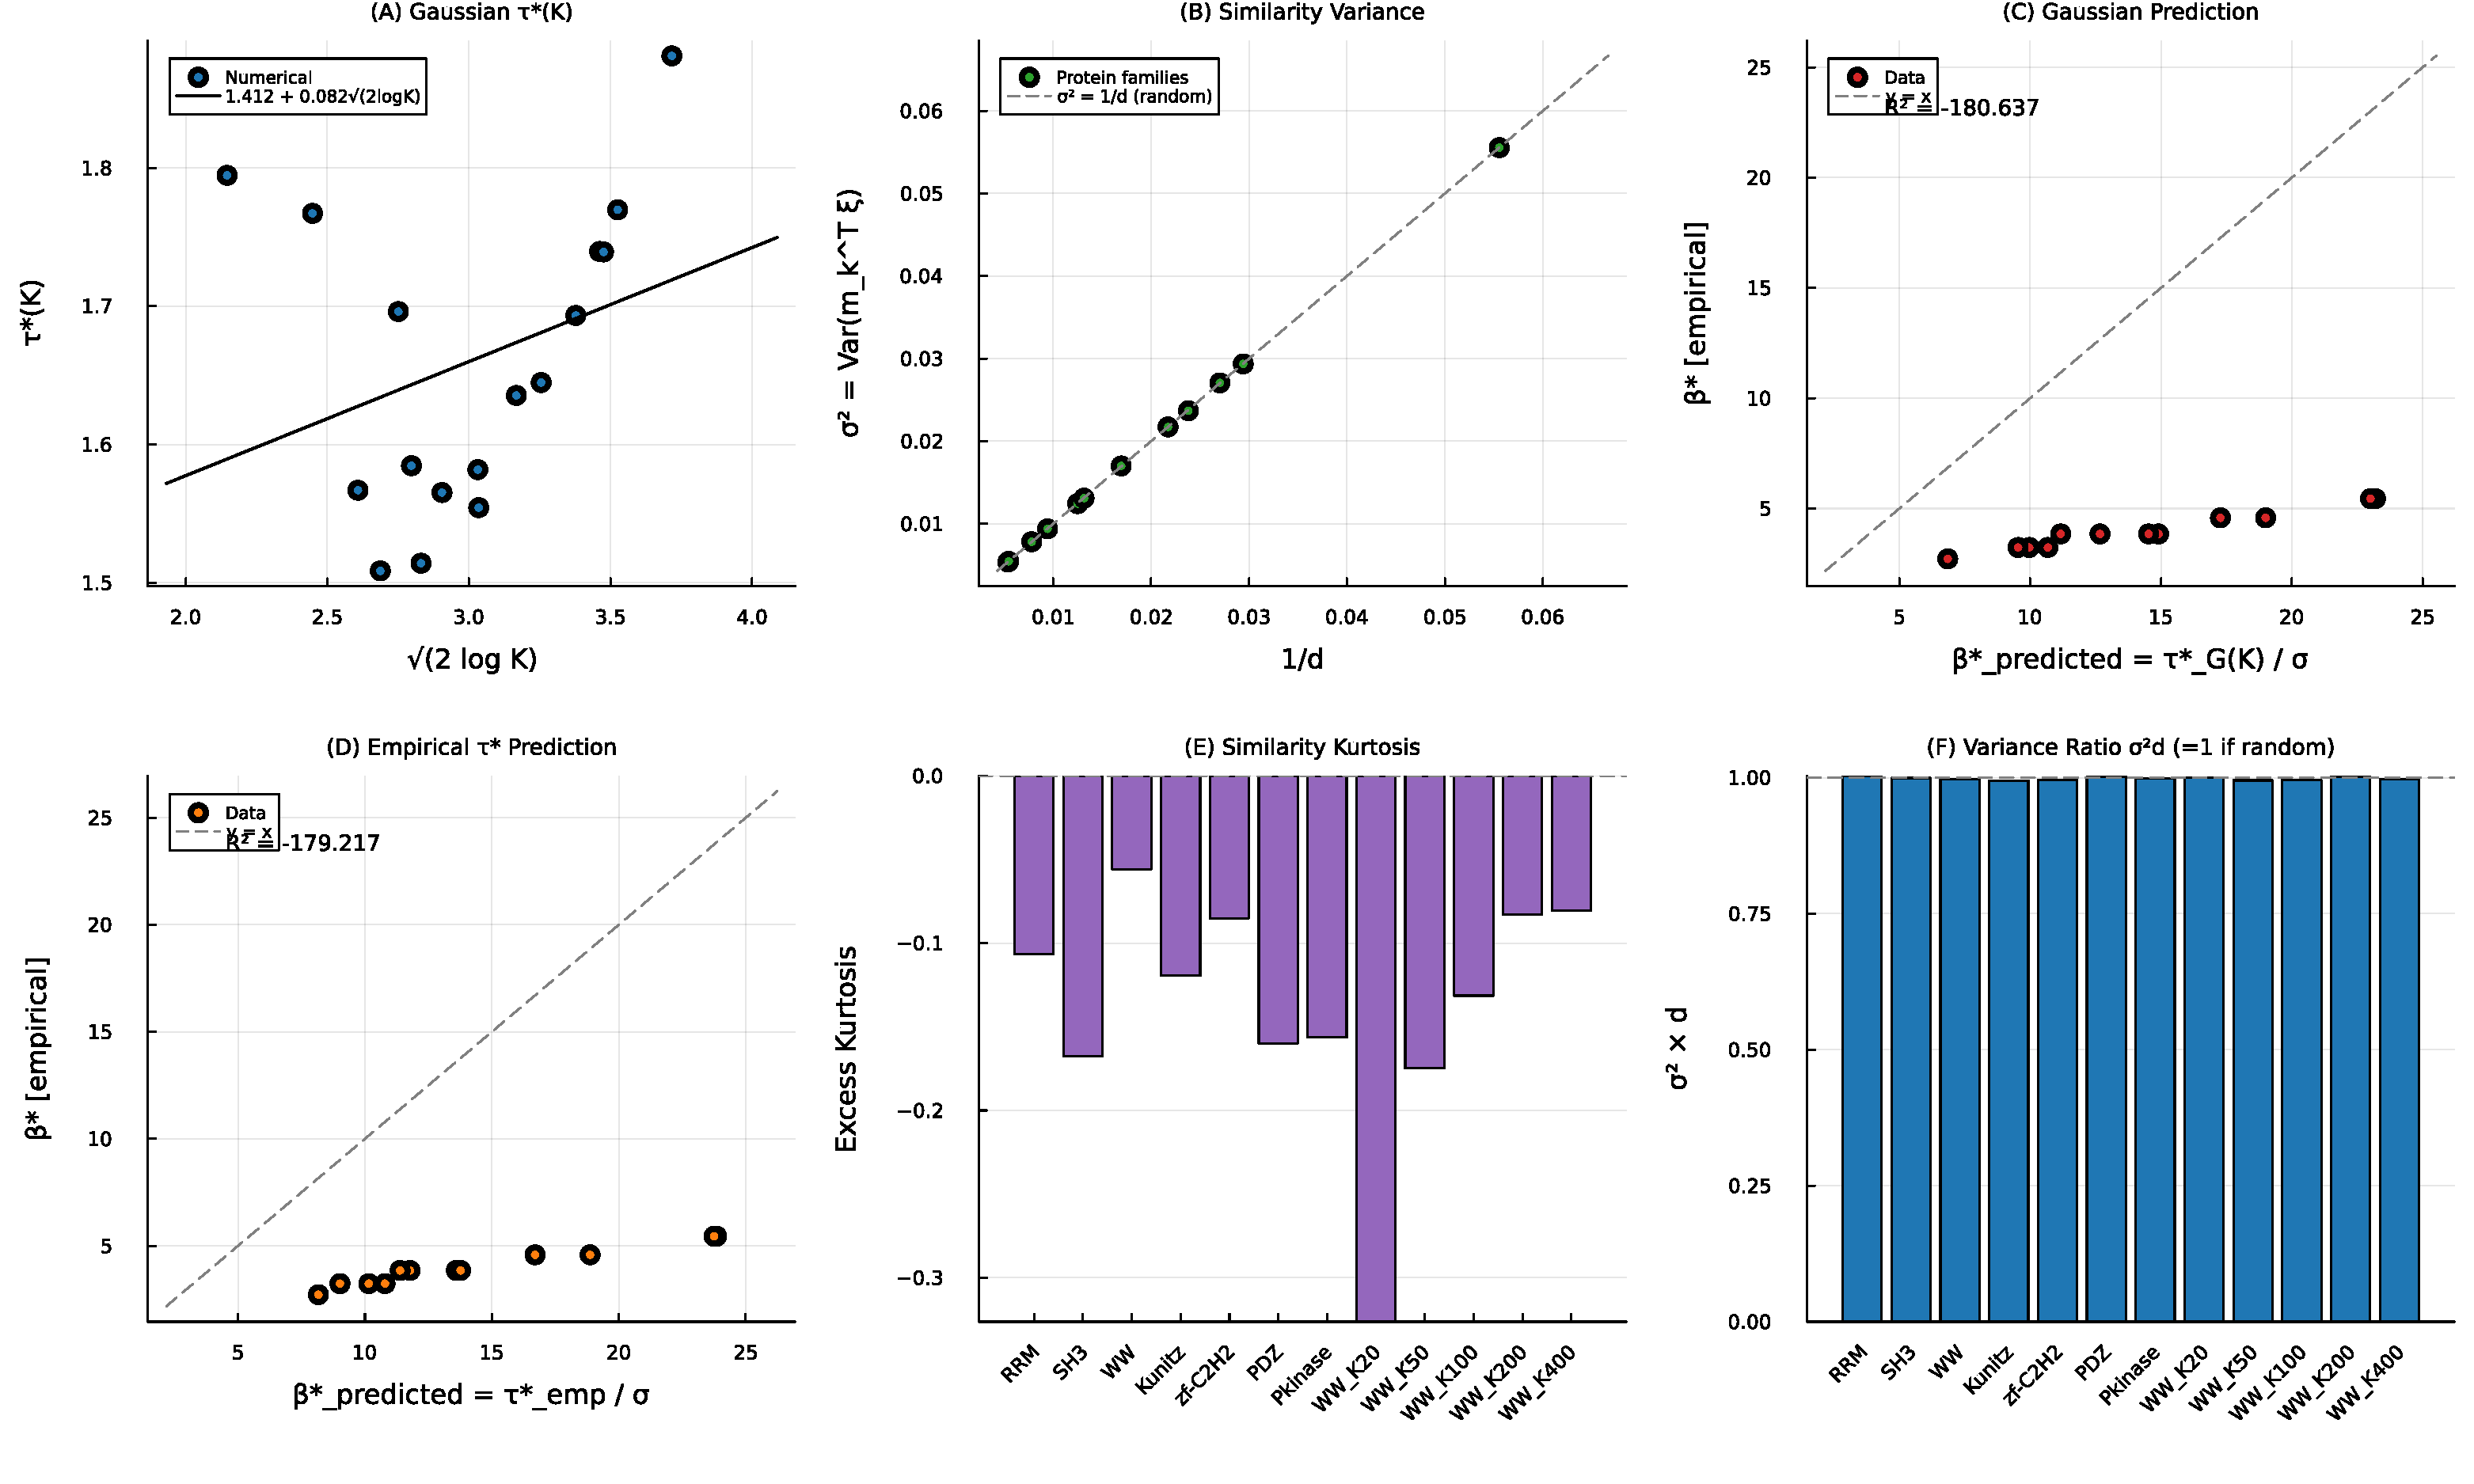
\includegraphics[width=0.7\textwidth]{figs/analytical_beta_star.pdf}
\caption{Analytical vs.\ empirical $\beta^*$.}
\label{fig:analytical-beta-star}
\end{figure}

\begin{figure}[ht]
\centering
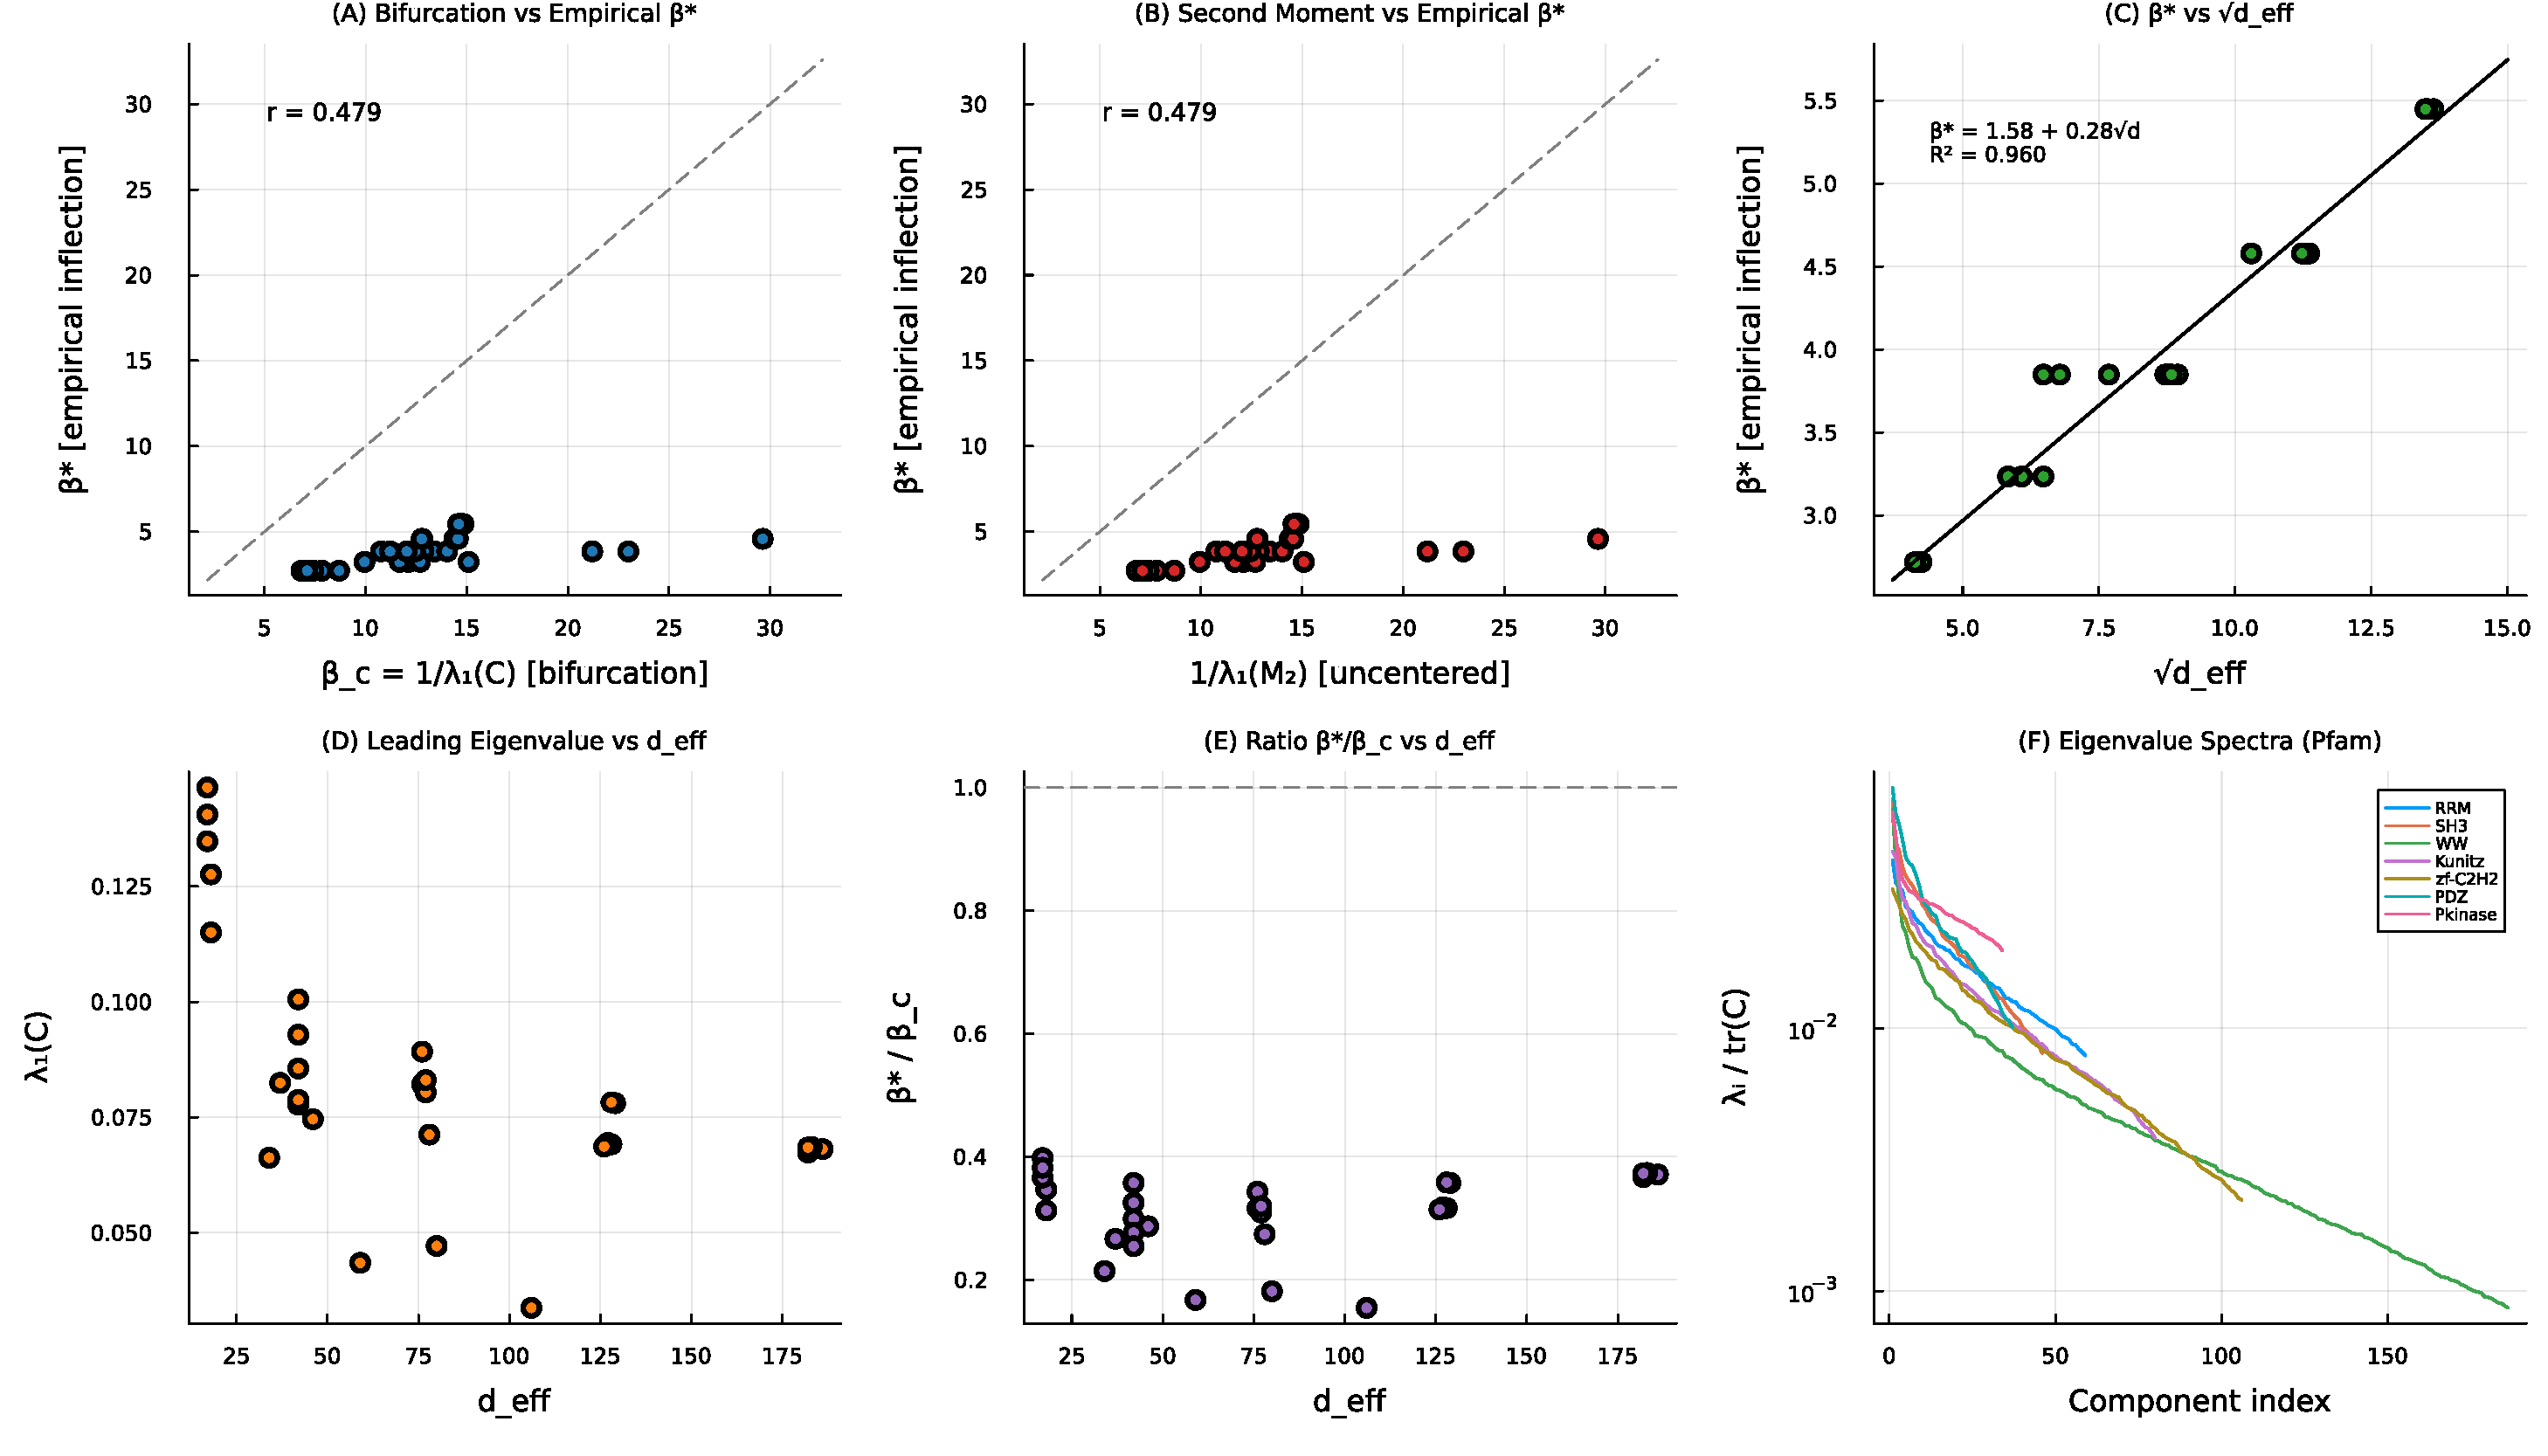
\includegraphics[width=0.7\textwidth]{figs/bifurcation_analysis.pdf}
\caption{Bifurcation analysis: $\beta_c = 1/\lambda_1(\mathbf{C})$ achieves only $r{=}0.48$.}
\label{fig:bifurcation-analysis}
\end{figure}

\begin{figure}[ht]
\centering
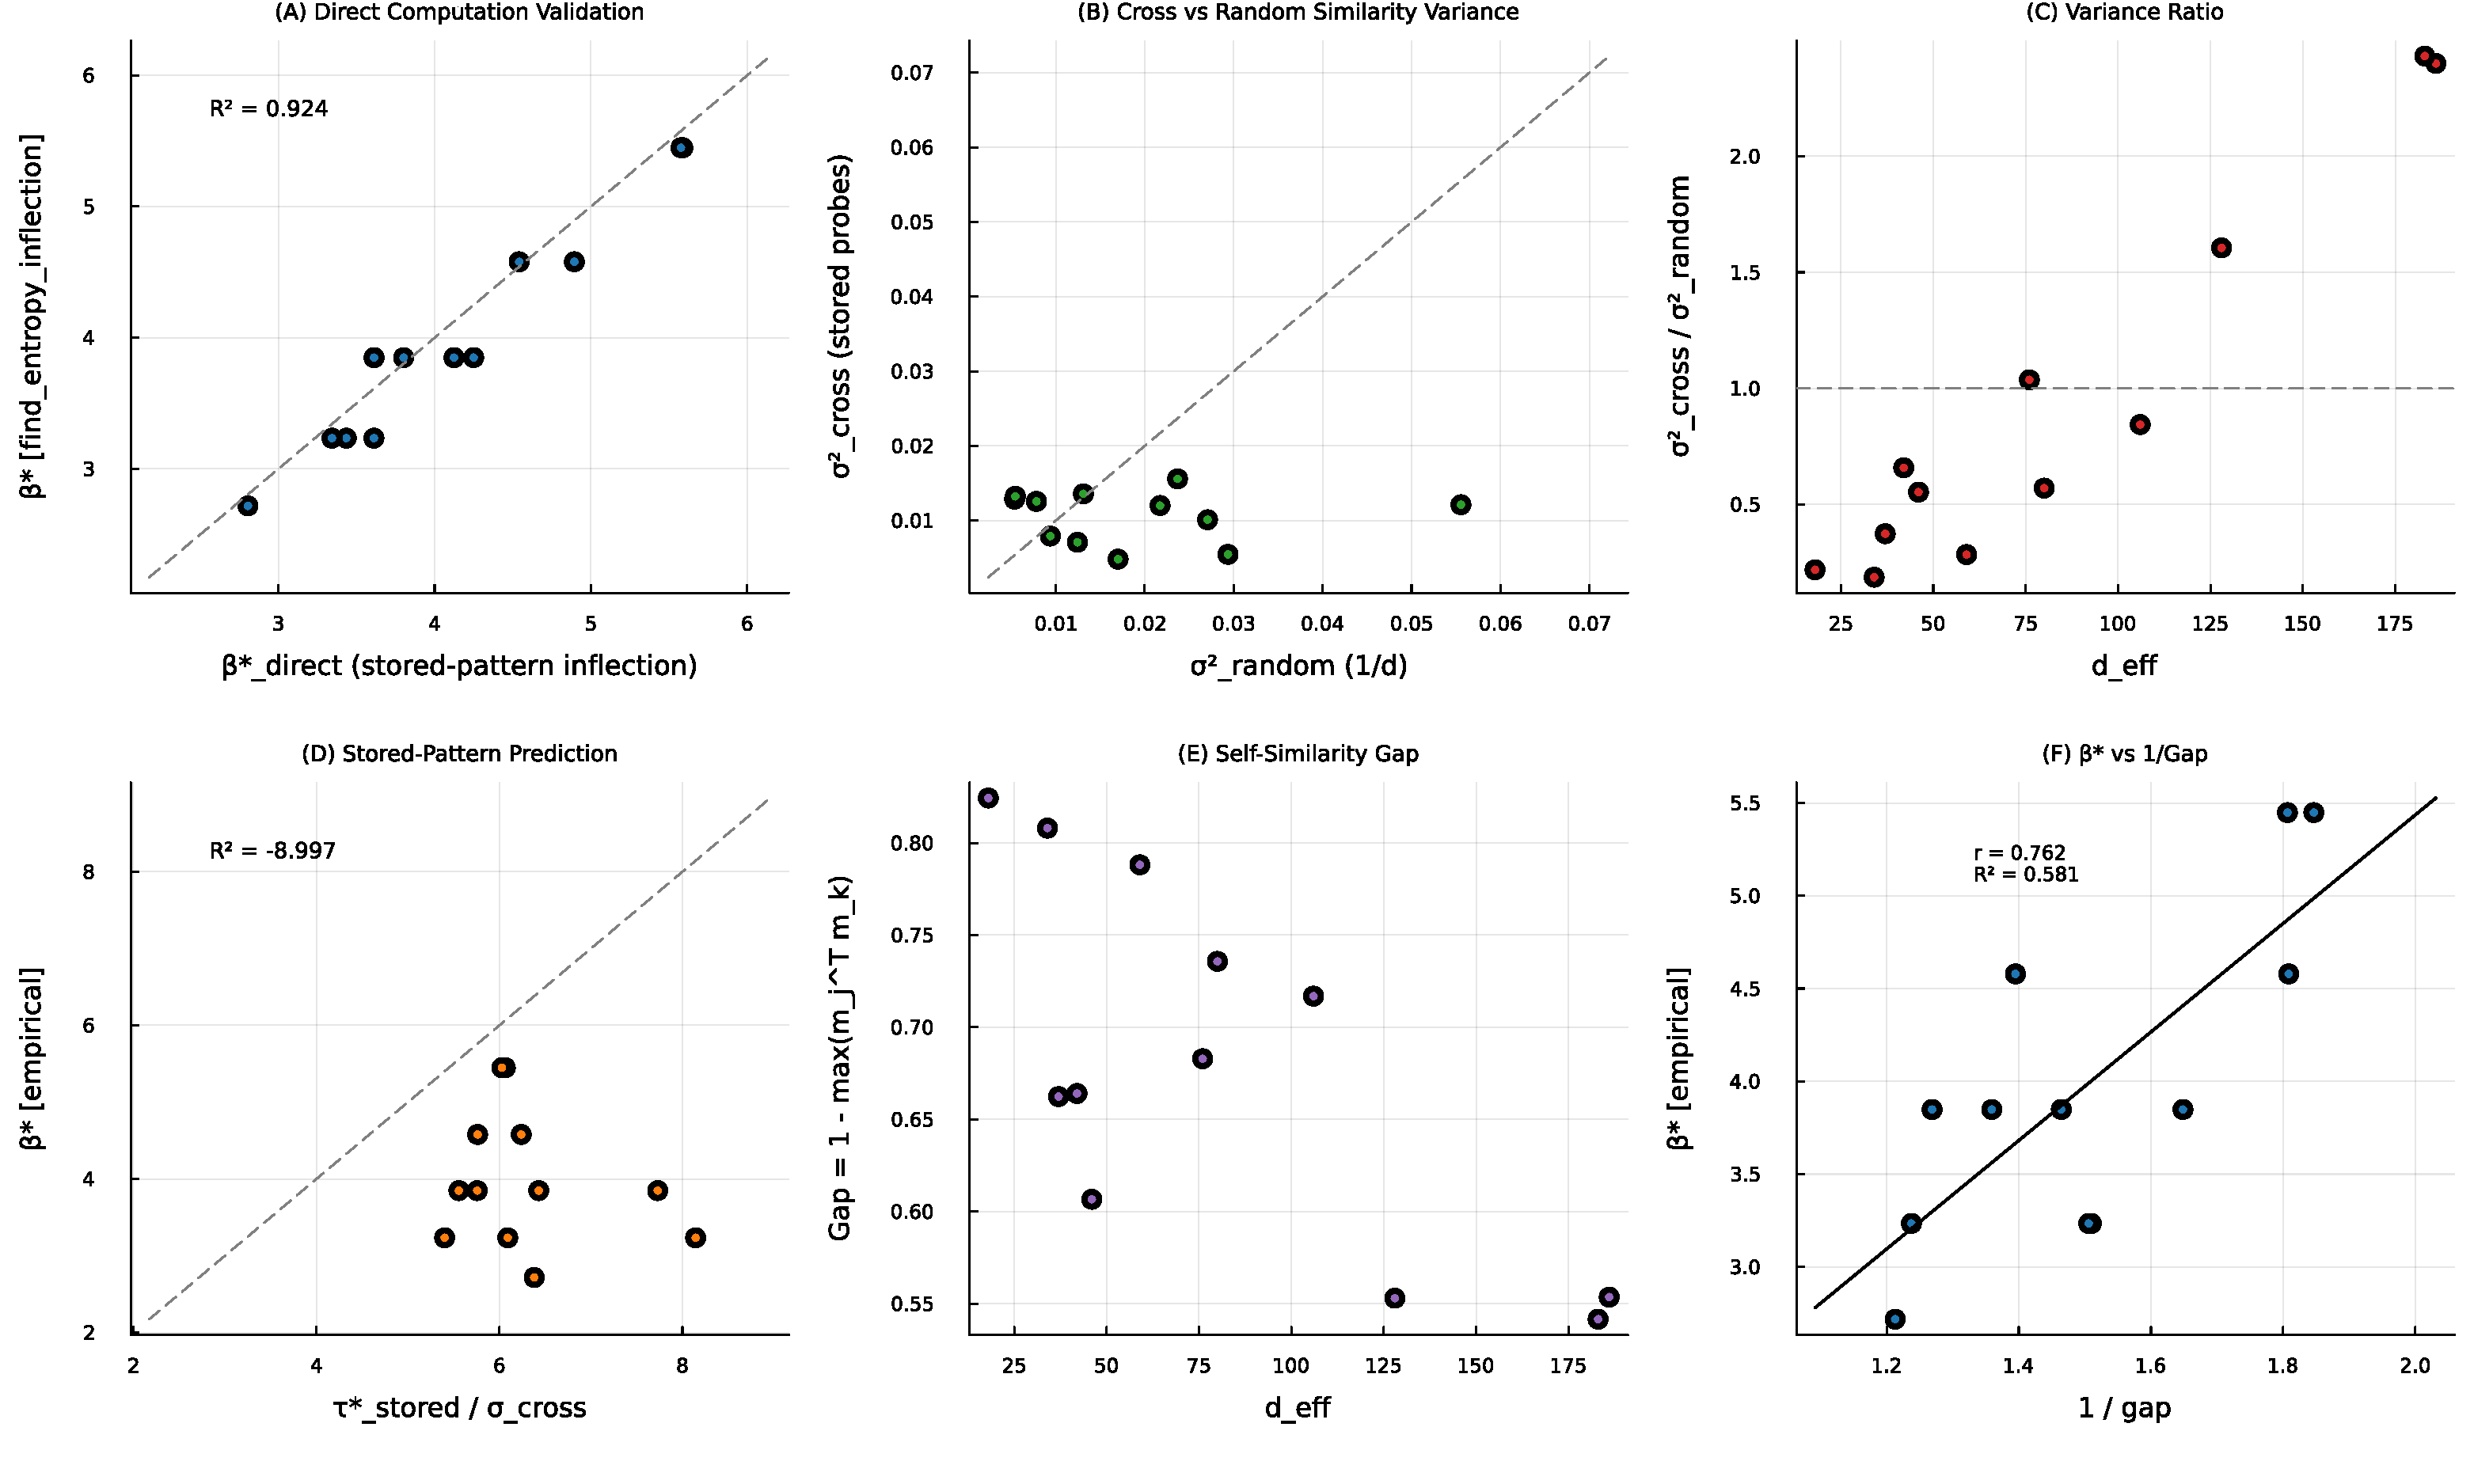
\includegraphics[width=0.7\textwidth]{figs/stored_pattern_analysis.pdf}
\caption{Stored-pattern analysis: self-similarity anchoring reduces the transition temperature relative to random-pattern predictions.}
\label{fig:stored-pattern-analysis}
\end{figure}

%% ═══════════════════════════════════════════════════════════════════════
%% S9. Theory Appendices (from original paper)
%% ═══════════════════════════════════════════════════════════════════════
\section{Concentration of Measure on the Sphere}\label{app:concentration}

Because the memory columns lie on the unit sphere $\mathbb{S}^{d-1}$, concentration of measure dictates that the similarity variance is $\mathrm{Var}(e_k) = 1/d$ exactly for any query drawn uniformly from $\mathbb{S}^{d-1}$. The characteristic similarity scale is therefore $\sigma = 1/\sqrt{d}$, and since $\beta$ enters the softmax as $\beta e_k$, the inflection must occur when $\beta\sigma = \mathcal{O}(1)$, giving $\beta^* \sim \sqrt{d}$.

\section{Universal Softmax Inflection}\label{app:tau-star}

The softmax entropy over $K$ i.i.d.\ Gaussian scores undergoes its inflection at a dimensionless temperature $\tau^* \approx 1.6$ that is nearly independent of $K$ for $K \geq 30$, providing a universal baseline for the transition.

\section{Stored-Pattern Probes}\label{app:stored-probes}

The coefficient $0.28$ of $\sqrt{d}$ is substantially smaller than the pure Gaussian prediction $\tau^*/\sigma \approx 1.6\sqrt{d}$; this reduction arises because $\beta^*$ is computed at stored patterns $\mathbf{m}_k$, where the self-similarity $\mathbf{m}_k^\top\mathbf{m}_k = 1$ anchors one score at the maximum of $\mathbb{S}^{d-1}$ and makes concentration easier than for a random query.

\section{Regularity and Convergence}\label{app:convergence}

The modern Hopfield energy has Lipschitz-continuous gradient with constant $L = 1 + \beta\sigma_{\max}^2/2$, where $\sigma_{\max} = \|\mathbf{X}\|_{\mathrm{op}}$, and satisfies the dissipativity condition $\langle \nabla E(\boldsymbol{\xi}), \boldsymbol{\xi} \rangle \geq \|\boldsymbol{\xi}\|^2/2 - M^2/2$ with $M = \max_k \|\mathbf{m}_k\|$. When $\beta\sigma_{\max}^2 < 2$, the energy is strictly convex and ULA iterates converge to $p_\beta$ in Wasserstein-2 distance at a geometric rate~\cite{dalalyanTheoreticalGuaranteesApproximate2017,durmusNonasymptoticAnalysisUnadjusted2017}. In the protein setting, operating temperatures satisfy $\beta\sigma_{\max}^2 \gg 2$, placing the sampler in a non-convex regime where the energy landscape has multiple metastable basins.

\section{OLS Regression for $\beta^*$}\label{app:beta-star-analysis}

Refitting the model on the eight Pfam families alone (excluding WW scaling replicates) yielded $\beta^* = 1.64 + 0.278\sqrt{d}$ ($R^2{=}0.95$), confirming that the result is not driven by overrepresentation of a single family.

%% ═══════════════════════════════════════════════════════════════════════
%% References
%% ═══════════════════════════════════════════════════════════════════════
\bibliographystyle{unsrtnat}
\bibliography{references}

\end{document}
